\documentclass[serif,xcolor=pdftex,dvipsnames,table,hyperref={bookmarks=false,breaklinks}]{beamer}

%%%%%%%%%%%%%%%%
% Change the macros below to configure the title slides
% for your course.
\newcommand{\coursename}{COMPSCI 589}
\newcommand{\instructor}{Benjamin M. Marlin}
\newcommand{\university}{University of Massachusetts Amherst}
\newcommand{\department}{College of Information and Computer Sciences}
%%%%%%%%%%%%%%%%


\newcommand{\settitlecard}[2]{
  \title[\coursename  Lecture #1] 
    {\coursename \\ Lecture #1: #2}
     \author[\instructor]{\instructor}
     \institute[\university]{
     \department\\
     \university
   }
\date{}
}

\newcommand{\maketitlepage}{
  \begin{frame}
  \titlepage
  \center{
    %If you use the slides unmodified, retain the attribution below
    \tiny{Slides by Benjamin M. Marlin (marlin@cs.umass.edu). \\
    \vspace{-1em}Created with support from National Science Foundation Award\# IIS-1350522. 
    %If you modify the slides, please retain the alternate attribution below
    %\tiny{Based on slides by Benjamin M. Marlin (marlin@cs.umass.edu). \\    
    %\vspace{-1em}Created with support from National Science Foundation Award\# IIS-1350522. 
    }                                              
  }  
  \end{frame}
}

\AtBeginSection[]
{
  \begin{frame}<beamer>{Outline}
    \tableofcontents[currentsection,subsectionstyle=hide]
  \end{frame}
}


\newcommand{\cut}[1]{}

\newcommand{\iconbox}[4]{
  \only<#1-#2>{
    \begin{columns}[T]
      \column{0.5in}
           \includegraphics[width=0.5in]{#3}
       \column{3.7in}
            #4
    \end{columns}
    \medskip
    \medskip
    \medskip
  }
}

\mode<presentation>{
  \usepackage{../beamertheme589theme}
  \setbeamercovered{invisible}
}

\mode<handout>{
  \usepackage{../beamertheme589theme}
  \setbeamercovered{transparent}
}


\usepackage[english]{babel}
\usepackage[latin1]{inputenc}
\usepackage{times}
\usepackage[T1]{fontenc}
\usepackage{amsmath}
\usepackage{amssymb}
\usepackage[noend]{algorithmic}
\usepackage{algorithm}
\usepackage{listings}

\renewcommand\mathfamilydefault{\rmdefault}

\newcommand{\setA}{\mathcal{A}}
\newcommand{\setB}{\mathcal{B}}
\newcommand{\setS}{\mathcal{S}}
\newcommand{\setV}{\mathcal{V}}
\DeclareMathOperator*{\union}{\bigcup}
\DeclareMathOperator*{\intersection}{\bigcap}
\DeclareMathOperator*{\Val}{Val}
\newcommand{\mbf}[1]{{\mathbf{#1}}}
\DeclareMathOperator*{\argmax}{arg\,max}
\DeclareMathOperator*{\argmin}{arg\,min}
\DeclareMathOperator*{\sign}{sign}
\newcommand{\deriv}[2]{\frac{\partial{#1}}{\partial{#2}}}


\settitlecard{7}{Ensembles and Classification}

\begin{document}

\maketitlepage


\section{Ensembles}
\subsection{Foo}

\begin{frame}[t]{Ensembles}

\begin{itemize}
\setlength{\itemsep}{8pt}

\item An \textit{ensemble} is simply a collection of models that are all trained to perform the same task. 

\pause\item An ensemble can consist of many different versions of the same model, or many different types of models.

\pause\item The final output for an ensemble of classifiers is typically obtained through a (weighted) average or vote of the predictions of the different models in the ensemble.

\pause\item An ensemble of different models that all achieve similar generalization performance often outperforms any of the individual models. 

\pause\item\textbf{Question:} How is this possible?

\end{itemize}

\end{frame}

\begin{frame}[t]{Ensemble Intuition}

\begin{itemize}
\setlength{\itemsep}{6pt}

\item Suppose we have an ensemble of binary classification functions $f_k(\mbf{x})$ for $k=1,...,K$.

\pause \item Suppose that on average they have the same expected error rate 
$\epsilon = E_{p(x,y)}[y\neq f_k(\mbf{x})]<0.5$, but that the errors they make are \textit{independent}. 

\pause\item The intuition is that the majority of the $K$ classifiers in the ensemble will be correct on many examples where any individual classifier makes an error. 

\pause \item A simple majority vote can significantly improve classification performance by \textit{decreasing variance} in this setting. 

\pause\item \textbf{Question:} How can we come up with such an ensemble?

\end{itemize}

\end{frame}

\begin{frame}[t]{Independent Training Sets}

\begin{itemize}
\setlength{\itemsep}{8pt}

\item Suppose we collect multiple independent training sets $Tr_1,...,Tr_K$ and use 
each of these training sets to train a different instance of the same classifier obtaining
$K$ classification functions $f_1(\mbf{x}),...,f_K(\mbf{x})$.

\pause\item Classifiers trained in this way are guaranteed to make independent errors on test data. 

\pause\item If the expected error of each classifier is less than $0.5$, then the weighted
majority vote is guaranteed to reduce the expected generalization error.

\pause\item \textbf{Question:} What is the weakness of this approach?
\end{itemize}

\end{frame}

\section{Bagging}
\subsection{Foo}

\begin{frame}[t]{Bagging}

\begin{itemize}
\setlength{\itemsep}{8pt}

\item Bootstrap aggregation or \textit{Bagging} is an approximation to the previous method that takes a single training set $Tr$ and randomly sub-samples from it $K$ times (with replacement) to form $K$ training sets $Tr_1,...,Tr_K$.

\pause\item Each of these training sets is used to train a different instance of the same classifier obtaining $K$ classification functions $f_1(\mbf{x}),...,f_K(\mbf{x})$.

\pause\item The errors won't by totally independent because the data sets aren't independent, but the random re-sampling usually introduces enough diversity to decrease the variance and give improved performance.

\end{itemize}

\end{frame}

\begin{frame}[t]{Bagging and Random Forests}

\begin{itemize}
\setlength{\itemsep}{8pt}

\item Bagging is particularly useful for high-variance, high-capacity models.

\pause\item Historically, it is most closely associated with decision tree models.

\pause\item A very successful extension of bagged trees is the random forest classifier.

\pause\item The random forests algorithm further decorrelates the learned trees by 
only considering a random sub-set of the available features when deciding which
variable to split on at each node in the tree.

\end{itemize}

\end{frame}

\begin{frame}[t]{Example: Bagging vs Random Forests}
\center
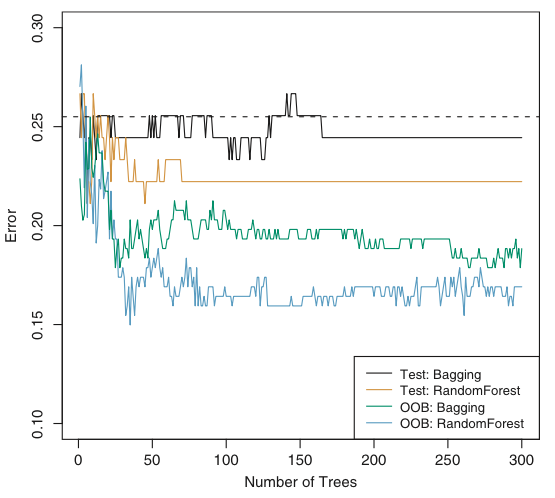
\includegraphics[width=3in]{../Figures/bagging_rf.png}
\end{frame}

\section{Boosting}
\subsection{Foo}


\begin{frame}[t]{Boosting}

\begin{itemize}
\setlength{\itemsep}{8pt}

\item Boosting is an ensemble method based on iteratively re-weighting the data set instead
of randomly resampling it.

\pause \item The main idea is to up-weight the importance of data cases that are missclassified by the classifiers currently in the ensemble, and then add a next classifier that will focus on data cases that are causing the errors.

\pause \item Assuming that the base classifier can always achieve an error of less than 0.5 on any data sample, the boosting ensemble can be shown to decrease error.

\end{itemize}

\end{frame}

\begin{frame}[t]{AdaBoost Algorithm}
\center
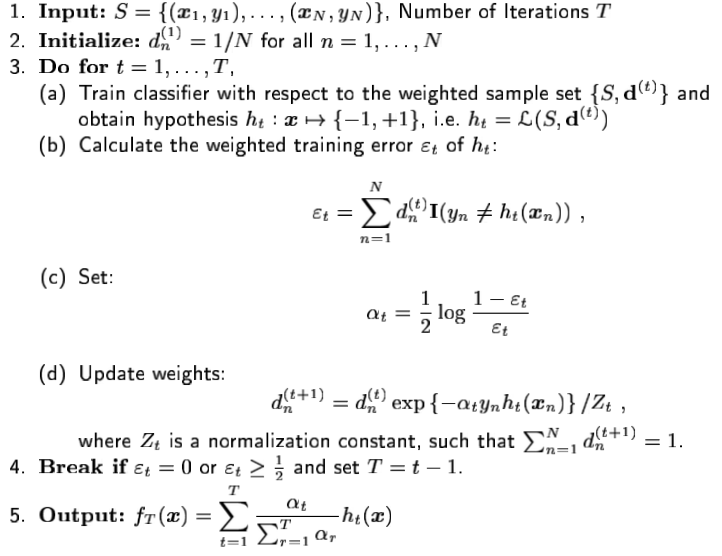
\includegraphics[width=3.5in]{../Figures/boosting_algorithm.png}
\end{frame}

\begin{frame}[t]{Example: AdaBoost}
\center
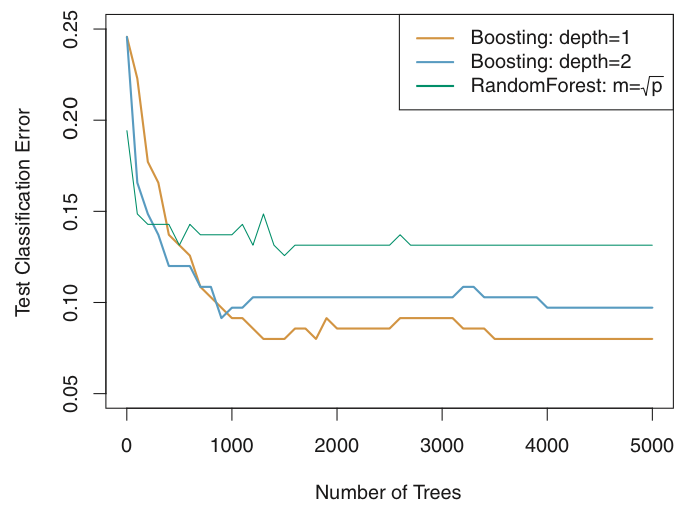
\includegraphics[width=3.5in]{../Figures/boosting_examples2.png}
\end{frame}

\section{Stacking}
\subsection{Foo}

\begin{frame}[t]{Stacking (or Blending)}

\begin{itemize}
\setlength{\itemsep}{8pt}

\item Unlike bagging and boosting, stacking is an algorithm for combining several different types of models.

\pause\item The main idea is to form a train-validation-test split and train many classifiers $f_k(\mbf{x})$ on the training data. 

\pause\item The trained classifiers are used to make predictions on the validation data set and
a new feature representation is then created where each data case consists of the vector of predictions of each classifier in the ensemble $\tilde{\mbf{x}} = [f_1(\mbf{x}),...,f_K(\mbf{x})]$.

\pause\item Finally, a meta-classifier called a \textit{combiner} is trained to minimize the validation error given the data $\{(y_i,\tilde{\mbf{x}}_i)|i=1,..,N\}$.

\pause\item The extra layer of combiner learning can deal with correlated classifiers as well 
as classifiers that perform poorly.

\end{itemize}
\end{frame}

\begin{frame}[t]{Example: Netflix Prize (2009)}
\vspace{-1em}
\center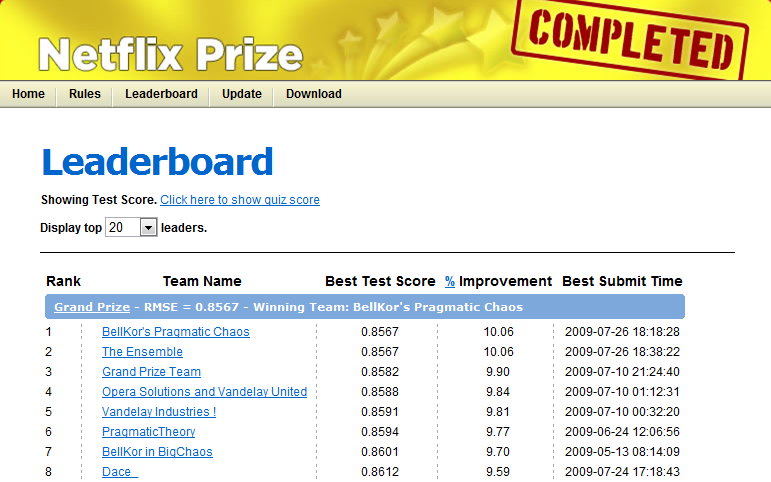
\includegraphics[width=4in]{../Figures/NetflixPrize.png}\\
\pause Winning team used stacked predictor of 450+ different models.
\end{frame}

\section{Wrap-Up}
\subsection{Foo}

\begin{frame}[t]{Classification Wrap-Up}

\begin{itemize}
\setlength{\itemsep}{8pt}

\item We've covered a good mix of classical and state-of-the-art classifiers including
KNN, decision trees, naive Bayes, LDA, logistic regression, SVMs, neural networks and
ensembles.

\pause\item We covered three of the most important meta issues in classification: generalization assessment, capacity control, and hyperparameter selection. 

\pause\item Things we didn't cover: feature selection, feature engineering, 
dealing with class imbalance, covariate shift, cost of errors, classifier evaluation beyond accuracy, structured prediction, sequential decisions...
\end{itemize}
\end{frame}

\begin{frame}[t]{Classifier Evaluation}
\center%
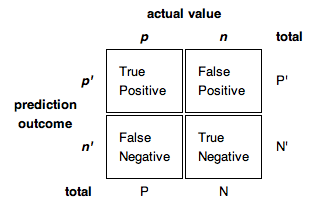
\includegraphics[width=3.5in]{../Figures/ConfusionMatrix.png}
\end{frame}

\begin{frame}[t]{Image Segmentation}
\center
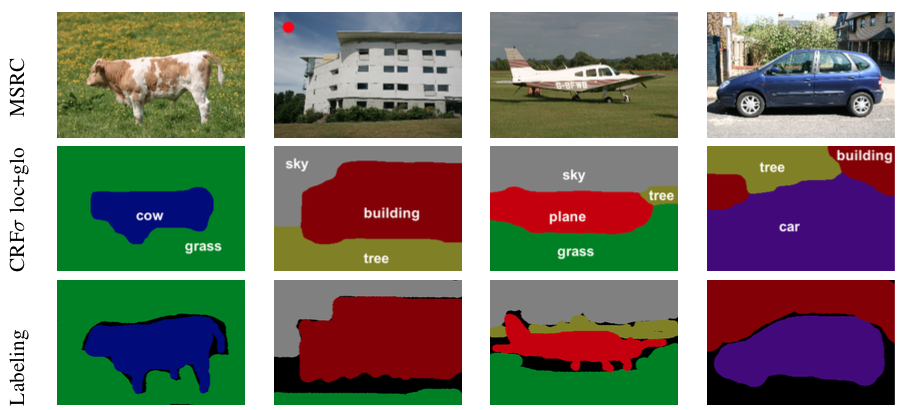
\includegraphics[width=4.5in]{../Figures/image_labeling.png}
\end{frame}

\begin{frame}[t]{Mesh Segmentation}
\center
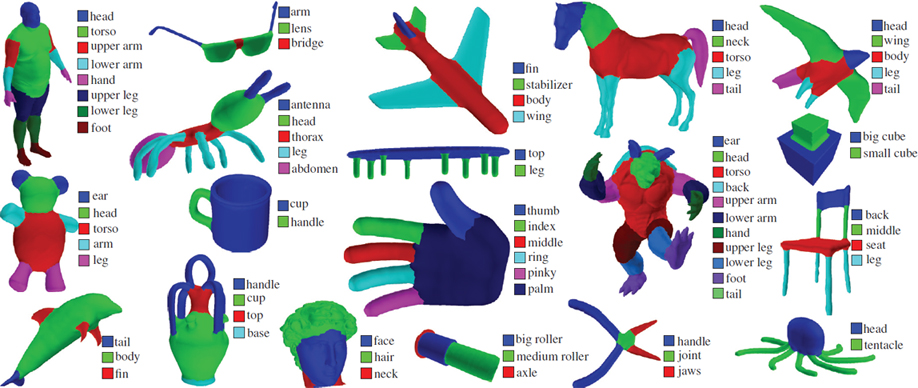
\includegraphics[width=4.5in]{../Figures/mesh_segmentation.jpg}
\end{frame}

\begin{frame}[t]{Image to Text}
\center

\includegraphics[width=3.5in]{../Figures/cat-hat.jpg}\\
\pause A very cute looking cat in a hat
\end{frame}

\begin{frame}[t]{Playing Atari Breakout}
\center
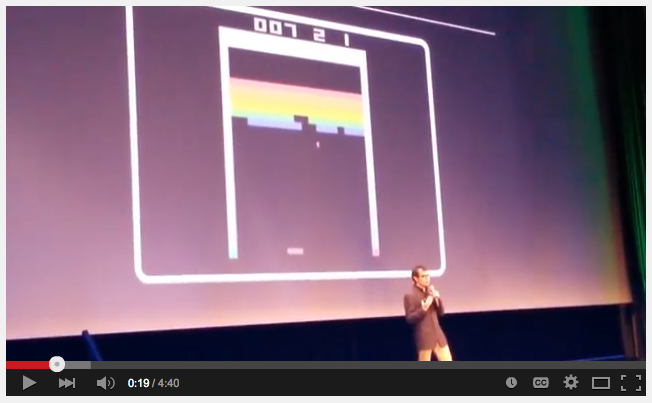
\includegraphics[width=3.5in]{../Figures/atari-nn.png}\\
\url{https://www.youtube.com/watch?v=EfGD2qveGdQ}
\end{frame}


\end{document}
